% !TeX root = ../solution.tex

\hypertarget{he22.17}{%
\chapter{[HE22.17] Crypto Bunny}\label{he22.17}}

\begin{marginfigure}
	
\includegraphics[width=49mm]{level5/challenge17.jpg}
\end{marginfigure}
\section{Intro}
View my verified achievement from (HOP)².

File: \verb+crypto_bunny.png+
\begin{marginfigure}
	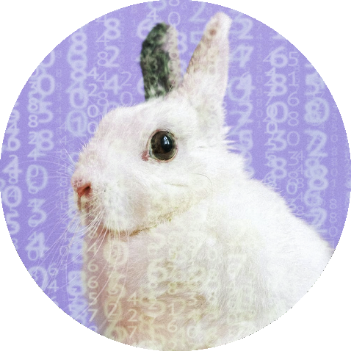
\includegraphics[width=50mm]{level5/crypto_bunny.png}
\end{marginfigure}
\section{Solution}\label{hv22.17solution}
Looking at the text in the file, it points towards badger.org and provides some information about the narrative:
going to \url{https://eu.badgr.com/public/badges/LaGEPKu1R2W5mg221vdV4g} gives us the hint that we have to solve the criteria.  

Rabbit ciper points towadrs \url{https://en.wikipedia.org/wiki/Rabbit_(cipher)}, an on-line solver at \url{https://www.browserling.com/tools/rabbit-decrypt} can be used to decode the ``narrative'' with the password \verb+carrot+, given as the tag.  The decoded message is \verb+Congrats, here's the flag: he2022{b4dg3_4w4rd3d}+

	









